%15 min preso!
\documentclass[xcolor=table,aspectratio=169]{beamer}
\usepackage{beamerthemesplit}
\usepackage{wrapfig}
\usetheme{SPbGU}
\usepackage{pdfpages}
\usepackage{amsmath}
\usepackage{cmap}
\usepackage[T2A]{fontenc}
\usepackage[utf8]{inputenc}
\usepackage[english]{babel}
\usepackage{indentfirst}
\usepackage{amsmath}
\usepackage{tikz}
\usepackage{multirow}
\usepackage[noend]{algpseudocode}
\usepackage{algorithm}
\usepackage{algorithmicx}
\usepackage{fancyvrb}
\usepackage{hyperref} 
\usetikzlibrary{calc}
\usetikzlibrary{shapes, backgrounds}
\usetikzlibrary{arrows,automata}
\usetikzlibrary{positioning}
\usetikzlibrary{fit}
\usetikzlibrary{shapes.callouts}
\usetikzlibrary{shapes.misc}
\usepackage{xparse}
\usepackage{fontawesome}
\usepackage{multicol}

\usepackage{etoolbox,refcount}
\usepackage{multicol}
\usepackage[export]{adjustbox}

\usepackage{tabularx}
\newcolumntype{Y}{>{\raggedleft\arraybackslash}X}

\renewcommand{\thealgorithm}{}

\newtheorem{mytheorem}{Theorem}
\renewcommand{\thealgorithm}{}

\newcommand{\tikzmark}[1]{\tikz[overlay,remember picture] \node (#1) {};}
\def\Put(#1,#2)#3{\leavevmode\makebox(0,0){\put(#1,#2){#3}}}

\newcommand{\ltz}{$< 1$}

\tikzset{
    state/.style={
           rectangle,
           rounded corners,
           draw=black, very thick,
           minimum height=2em,
           inner sep=2pt,
           text centered,
           },
}

\tikzset{
    invisible/.style={opacity=0,text opacity=0},
    visible on/.style={alt=#1{}{invisible}},
    alt/.code args={<#1>#2#3}{%
      \alt<#1>{\pgfkeysalso{#2}}{\pgfkeysalso{#3}} % \pgfkeysalso doesn't change the path
    },
}

\tikzset{cross/.style={cross out, draw=black, minimum size=2*(#1-\pgflinewidth), inner sep=0pt, outer sep=0pt, ultra thick},
%default radius will be 1pt. 
cross/.default={1pt}}

\NewDocumentCommand{\mycallout}{r<> O{opacity=0.8,text opacity=1} m m m}{%
\tikz[remember picture, overlay]\node[align=center, fill=cyan!20, text width=#5cm,
#2,visible on=<#1>, rounded corners,
draw,rectangle callout,anchor=pointer,callout relative pointer={(290:0.5cm)}]
at (#3) {#4};
}

\NewDocumentCommand{\mycalloutR}{r<> O{opacity=0.8,text opacity=1} m m m}{%
\tikz[remember picture, overlay]\node[align=center, fill=cyan!20, text width=#5cm,
#2,visible on=<#1>, rounded corners,
draw,rectangle callout,anchor=pointer,callout relative pointer={(30:0.8cm)}]
at (#3) {#4};
}


%callout relative pointer={(230:0.5cm)}]

\newcounter{countitems}
\newcounter{nextitemizecount}
\newcommand{\setupcountitems}{%
  \stepcounter{nextitemizecount}%
  \setcounter{countitems}{0}%
  \preto\item{\stepcounter{countitems}}%
}
\makeatletter
\newcommand{\computecountitems}{%
  \edef\@currentlabel{\number\c@countitems}%
  \label{countitems@\number\numexpr\value{nextitemizecount}-1\relax}%
}
\newcommand{\nextitemizecount}{%
  \getrefnumber{countitems@\number\c@nextitemizecount}%
}
\newcommand{\previtemizecount}{%
  \getrefnumber{countitems@\number\numexpr\value{nextitemizecount}-1\relax}%
}
\makeatother    
\newenvironment{AutoMultiColItemize}{%
\ifnumcomp{\nextitemizecount}{>}{3}{\begin{multicols}{2}}{}%
\setupcountitems\begin{itemize}}%
{\end{itemize}%
\unskip\computecountitems\ifnumcomp{\previtemizecount}{>}{3}{\end{multicols}}{}}


\beamertemplatenavigationsymbolsempty

\title[GPGPU + OpenCL]{Особенности разработки под графические ускорители на примере OpenCL: от архитектуры вычислителя до особенностей оптимизации}
\institute[СПбГУ]{Снакт-Петербургский Государственный Университет
}

% То, что в квадратных скобках, отображается в левом нижнем углу.
\author[Семён Григорьев]{Семён Григорьев}

\date{27 января 2025}


\begin{document}
{
\begin{frame}[fragile]
  \begin{table}
  \centering
  %
\includegraphics[height=1.5cm]{pictures/SPbGU_Logo.png}
  \begin{tabularx}{\linewidth}{XcX}
    %\includegraphics[height=1.6cm]{pictures/} 
    \hfill
    & 
    & \hfill 
\includegraphics[height=1.6cm]{pictures/SPbGU_Logo.png}
  \end{tabularx}
  \end{table}
  \titlepage
\end{frame}
}

\begin{frame}[fragile]
  \frametitle{Семён Григорьев}
  \begin{minipage}{0.70\textwidth}
  \begin{itemize}    
    \item Доцент кафедры системного программирования Санкт-Петербургского Государственного Университета
    \item Области интересов
    \begin{itemize}    
      \item \textbf{Высокопроизводительный анализ графов}
      \begin{itemize}    
        \item В том числе, с использованием \textbf{графических ускорителей}
      \end{itemize}
      \item \textbf{Высокопроизводительная линейная алгебра} для анализа графов
      \begin{itemize}    
        \item \textbf{Обобщённая}: матрицы и вектора параметризованы типом элемента, операции над ними могут быть заданы пользователем
        \item \textbf{Разреженная}: специализированные структуры для хранения матриц и векторов, специализированные алгоритмы для их обработки 
        \item В том числе, с использованием \textbf{графических ускорителей}
      \end{itemize}
      \item Высокоуровневые средства разработки для графических ускорителей      
    \end{itemize}
    \end{itemize}
\end{minipage}
\begin{minipage}[t]{0.29\textwidth}
  \begin{center}
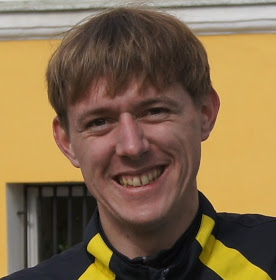
\includegraphics[width=0.8\textwidth]{pictures/SemyonGrigorev.jpg}
  \end{center}
  {\scriptsize
\begin{itemize}    
  \item Email: rsdpisuy@gmail.com 
  \item GitHub: \href{https://github.com/gsvgit}{gsvgit}
  \item Google Scholar: \href{https://scholar.google.com/citations?hl=ru&user=kP4dqUAAAAAJ&view_op=list_works&sortby=pubdate}{Semyon Grigorev}
  \item DBLP: \href{https://dblp.org/pid/181/9903.html}{Semyon V. Grigorev}
\end{itemize}
  }
\end{minipage}
\end{frame}

\begin{frame}[fragile]
  \frametitle{План лекции}
  \underline{\textbf{Цель лекции:}} познакомить с графическими ускорителями, показать, на что стоит обращать внимание при первых попытках программировать под них
  \vfill
  \begin{enumerate}
    \item Параллельность: что, зачем, какая бывает, какая нас будет интересовать
    \item CPU и GPGPU: сходства, различия, взаимосвязь
    \item Основные принципы архитектуры  GPGPU
    \item Основы OpenCL
    \item Немного про оптимизации для GPGPU
  \end{enumerate}
\end{frame}


\begin{frame}[fragile]
  \frametitle{Параллелизм}
  \begin{center}
    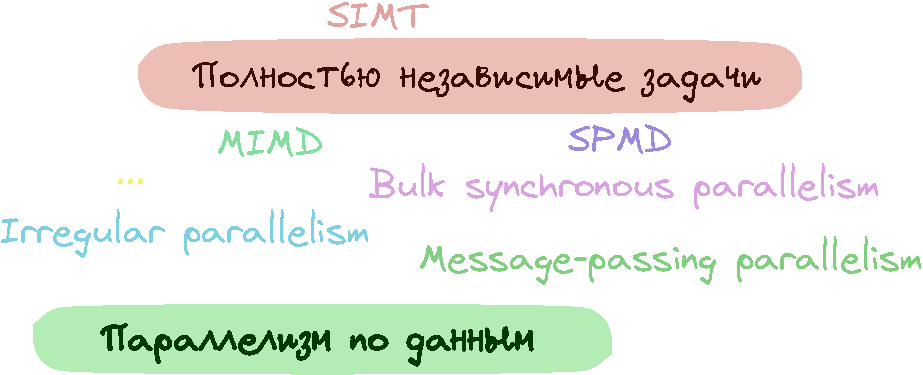
\includegraphics[width=0.8\textwidth]{pictures/parallel_types_crp.pdf}
  \end{center}
\end{frame}


\begin{frame}[fragile]
  \frametitle{Параллелизм по данным}
    \begin{itemize}
      \item Одна и та же функция применяется \textbf{независимо} ко всем элементам набора данных\footnote{Можно представить map, iter и прочие аналоги на коллекциях}
      \begin{center}
        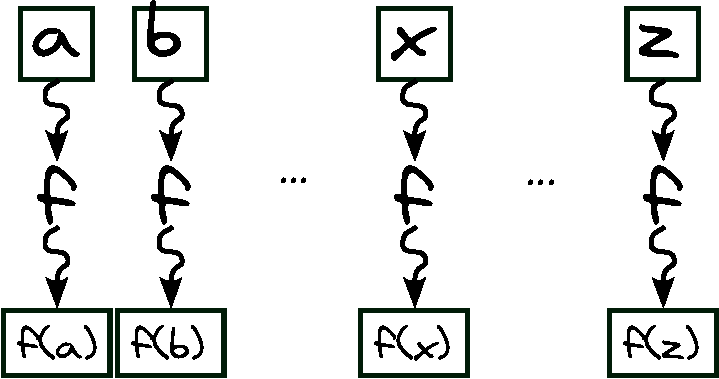
\includegraphics[height=2cm]{pictures/simd_crp.pdf}
      \end{center}
    \item Single Instruction Multiple Data (SIMD)
    \begin{itemize}
      
      \item Не функция, но \textbf{инструкция}: поток управления функции должен быть максимально простым
      \begin{itemize}
        \item[$\Rightarrow$] Много ветвлений --- \textbf{плохо}\footnote{Современные GPGPU стараются бороться с этим ограничением}
        \item[$\Rightarrow$] Много однотипных вычислений --- \textbf{хорошо}
        \item[$\Rightarrow$] Данные должны быть \textbf{однородными}
      \end{itemize}
      \item Типично для обработки изображений, линейной алгебры
      \begin{itemize}
        \item Вектора, матрицы --- хорошие массивы данных
        \item Много вычислительно интенсивной, но <<однотипной>> работы
      \end{itemize}
  \end{itemize}
\end{itemize}
  
\end{frame}


\begin{frame}[fragile]
  \begin{minipage}[t]{0.49\textwidth}
    \textbf{CPU}
    \begin{itemize}
      \item Процессор общего назначения
      \item Независимые задачи
      \item Много сложных кэшей
      \item Сложный поток управления
    \end{itemize}
  \end{minipage}
  \begin{minipage}[t]{0.49\textwidth}
    \textbf{GPGPU}
    \begin{itemize}
      \item Специализированный \underline{\textbf{(со)}}процессор
      \item Параллелизм по данным
      \item Высокая пропускная способность
      \item Большое количество простых ALU
    \end{itemize}
  \end{minipage}
\\
  \begin{center}
    Типичный <<взгляд издалека>>\\
    \begin{minipage}[t]{0.49\textwidth}
      \begin{center}
      Сравнение архитектур\footnotemark[3]
    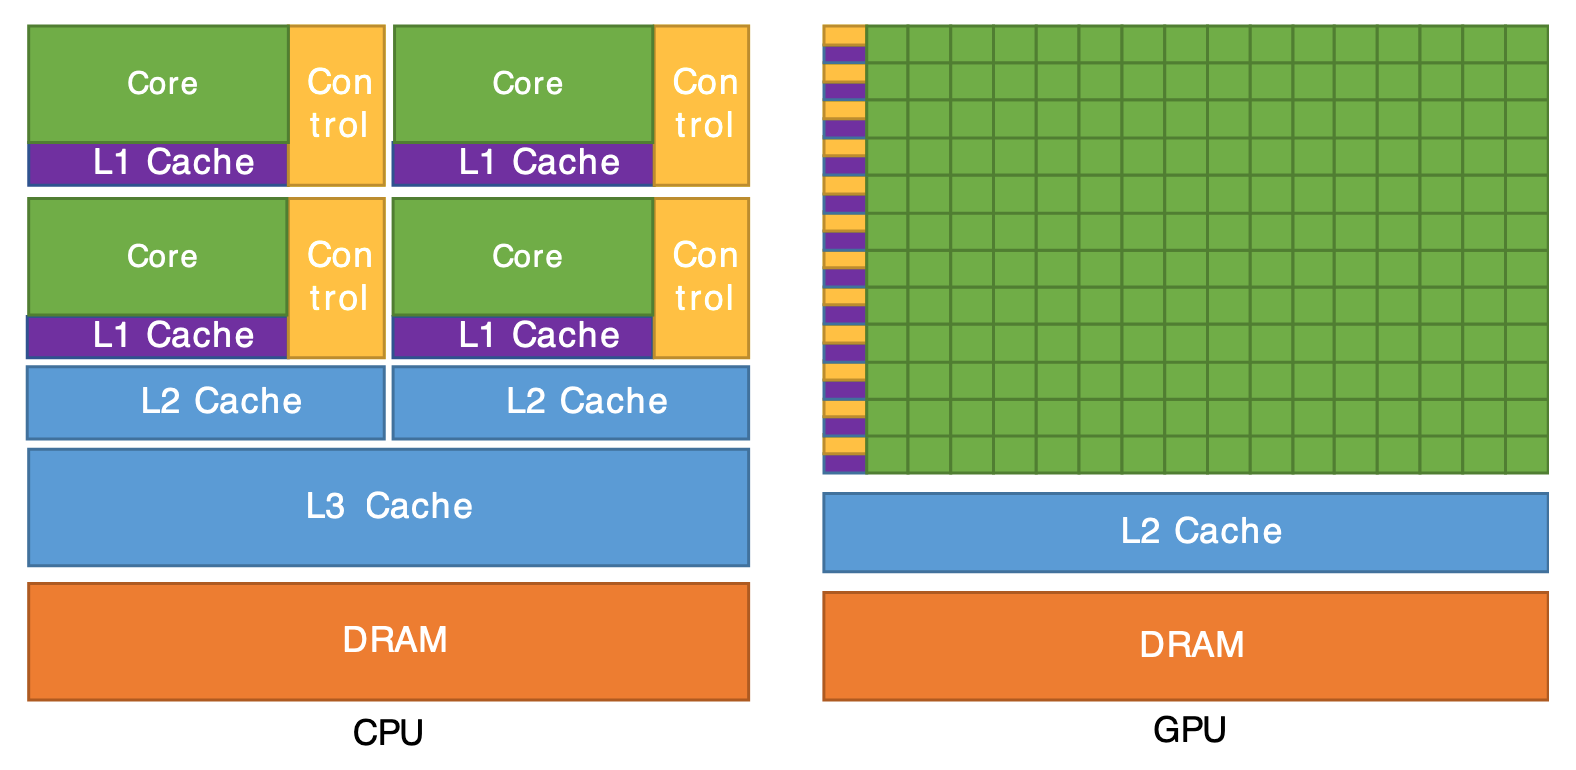
\includegraphics[width=0.99\textwidth]{pictures/ArchCPUGPUcores.png}
      \end{center}
    \end{minipage}
    \begin{minipage}[t]{0.49\textwidth}
      \begin{center}
      Взаимодействие в SoC\footnotemark[4]
    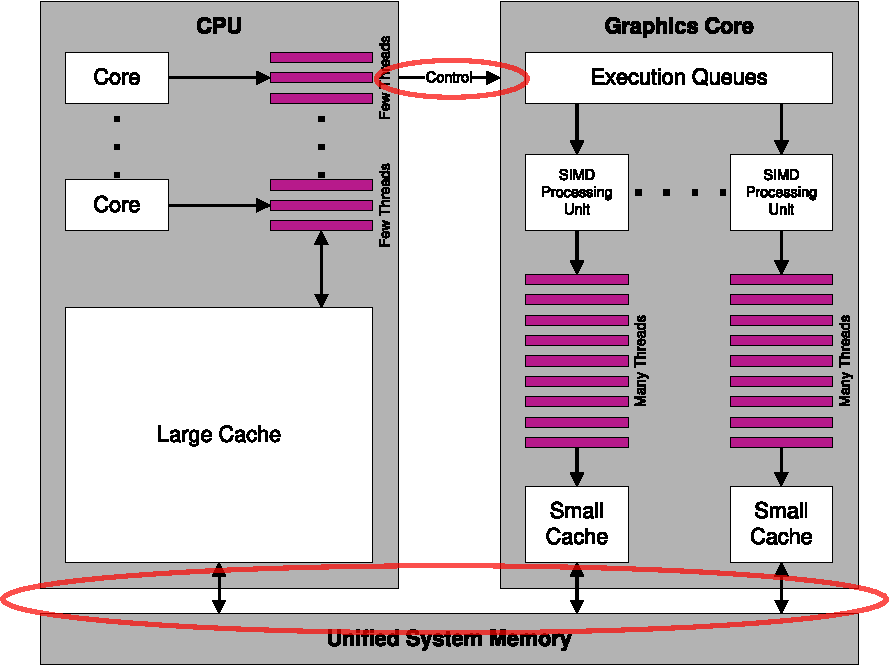
\includegraphics[width=0.7\textwidth]{pictures/SoC_GPU_crp.pdf}
      \end{center}
  \end{minipage}
  \end{center}
  \footnotetext[3]{\url{https://cvw.cac.cornell.edu/gpu-architecture/gpu-characteristics/design}}
  \footnotetext[4]{PowerVR Hardware. Architecture Overview for Developers}
\end{frame}

\setcounter{footnote}{4}

\begin{frame}[fragile]
  \frametitle{Проблемы\footnote{как всегда, в деталях}}
  \begin{itemize}
    \item Масса вендоров:
    \begin{multicols}{3}
    \begin{itemize}
      \item Nvidia
      \item AMD
      \item Intel
      \item Imagination Technologies
      \item Qualcomm
      \item \ldots
    \end{itemize}
  \end{multicols}
    \item Микроархитектура различных графических ускорителей сильно различается
    \item Архитектура различных графических ускорителей сильно различается
    \item Терминология сильно различается
  \end{itemize}
  \begin{center}
  \begin{tabular}{ c c c c}
    \rowcolor{lightgray}
    Nvidia & AMD & Intel & Im.Tech. \\ 
    \hline
    \hline
    Streaming Processor      & SIMD lane      & Processing element & ALU Group               \\  
    \rowcolor{lightgray}
    SIMT unit                & SIMD unit      & Vector engine      & ALU Pipeline            \\
    Streaming Multiprocessor & Computing Unit & Execution Unit     & Unified Shading Cluster \\
    \rowcolor{lightgray}
    GPU processing clusters  & Compute Engine & Xe-slice           & Core
   \end{tabular}
  \end{center}
\end{frame}

\begin{frame}[fragile]
  \frametitle{Интегрированная графика от Intel\footnote{Древняя, Gen11}\textsuperscript{,}\footnote{Изображения из <<Intel\textsuperscript{\textregistered} Processor Graphics Gen11
  Architecture>>}}
  \begin{minipage}[t]{0.32\textwidth}
  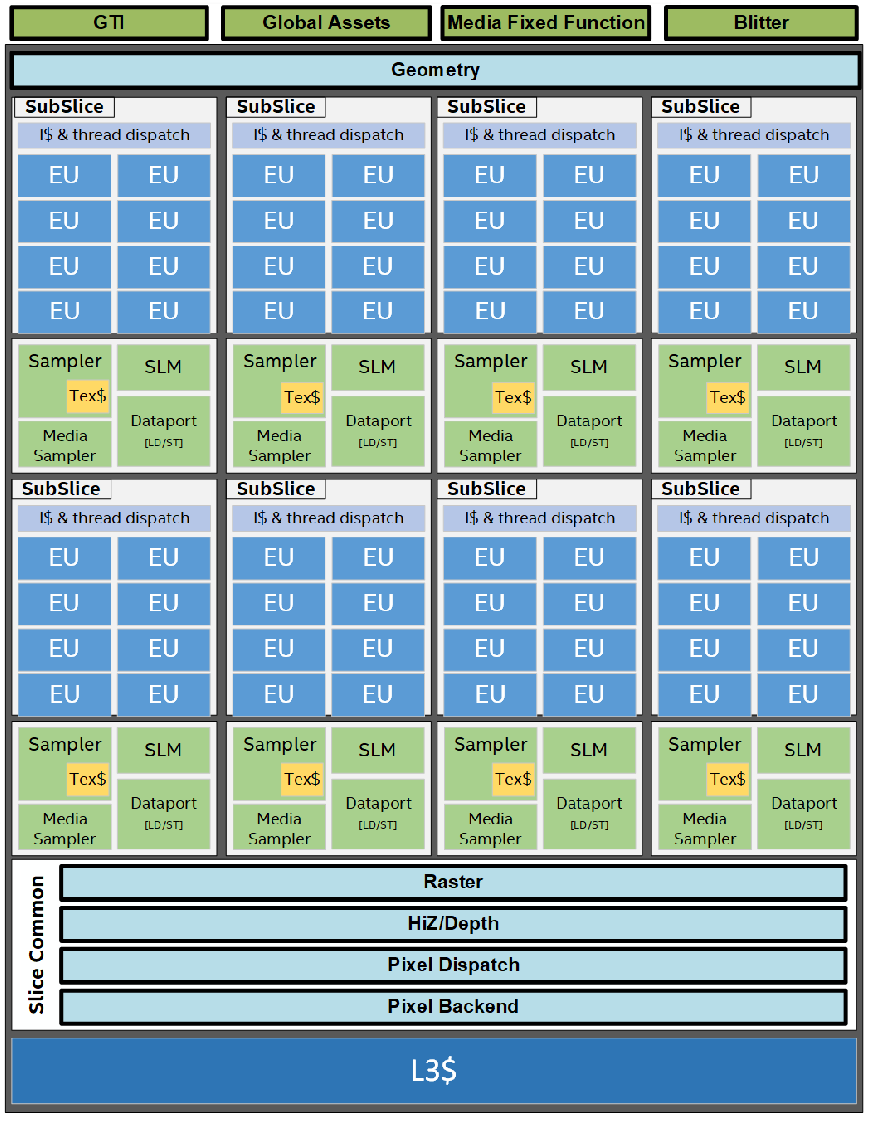
\includegraphics[valign=t,width=\textwidth]{pictures/intel_gpu_crp.pdf}
  \end{minipage}
  \begin{minipage}[t]{0.27\textwidth}
  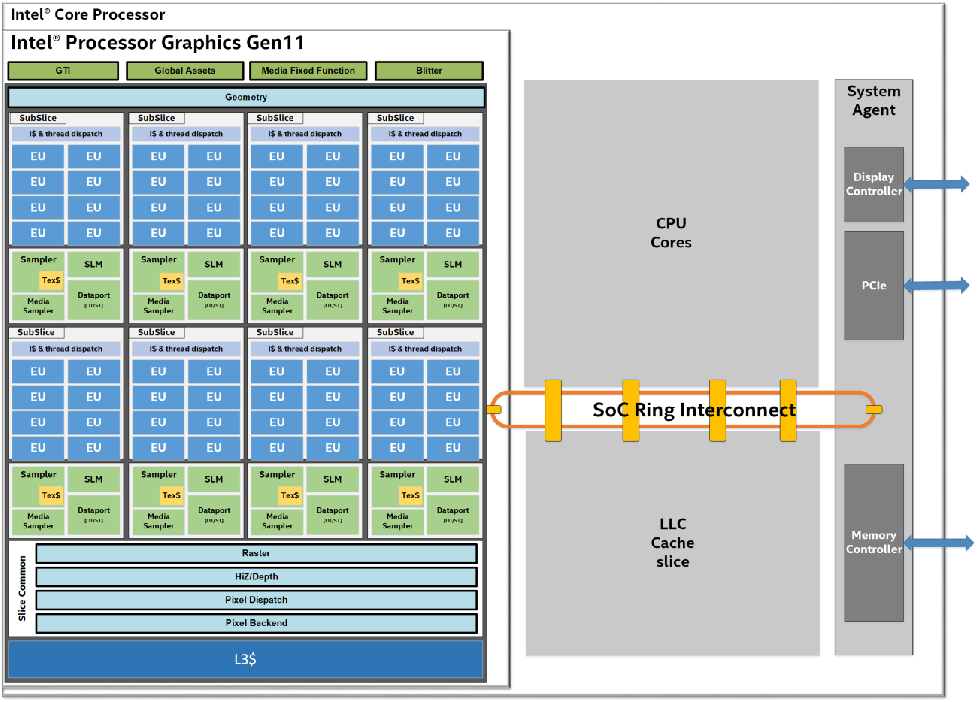
\includegraphics[valign=t,width=\textwidth]{pictures/intel_gpu_and_cpu_crp.pdf}
  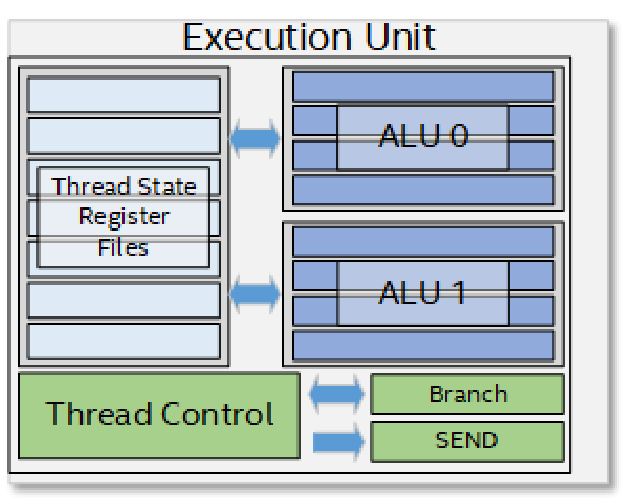
\includegraphics[valign=b,width=\textwidth]{pictures/intel_execution_unit_crp.pdf}
  \end{minipage}
  \begin{minipage}[t]{0.37\textwidth}
    \begin{itemize}
      \item Много специфики по обработке изображений
      \item Иерархическая группировка элементов
      \item Общий с процессором кэш
    \end{itemize}
    \end{minipage}
\end{frame}

\begin{frame}[fragile]
  \frametitle{Графичекий ускоритель от Imagination Technologies (PowerVR)\footnote{Примерно то, с чем некоторые столкнутся на школе}\textsuperscript{,}\footnote{Изображения из документации: \url{https://docs.imgtec.com/performance-guides/compute-recommendations/html/topics/architecture/overview.html}}}
  \begin{minipage}[t]{0.49\textwidth}
    \begin{center}
  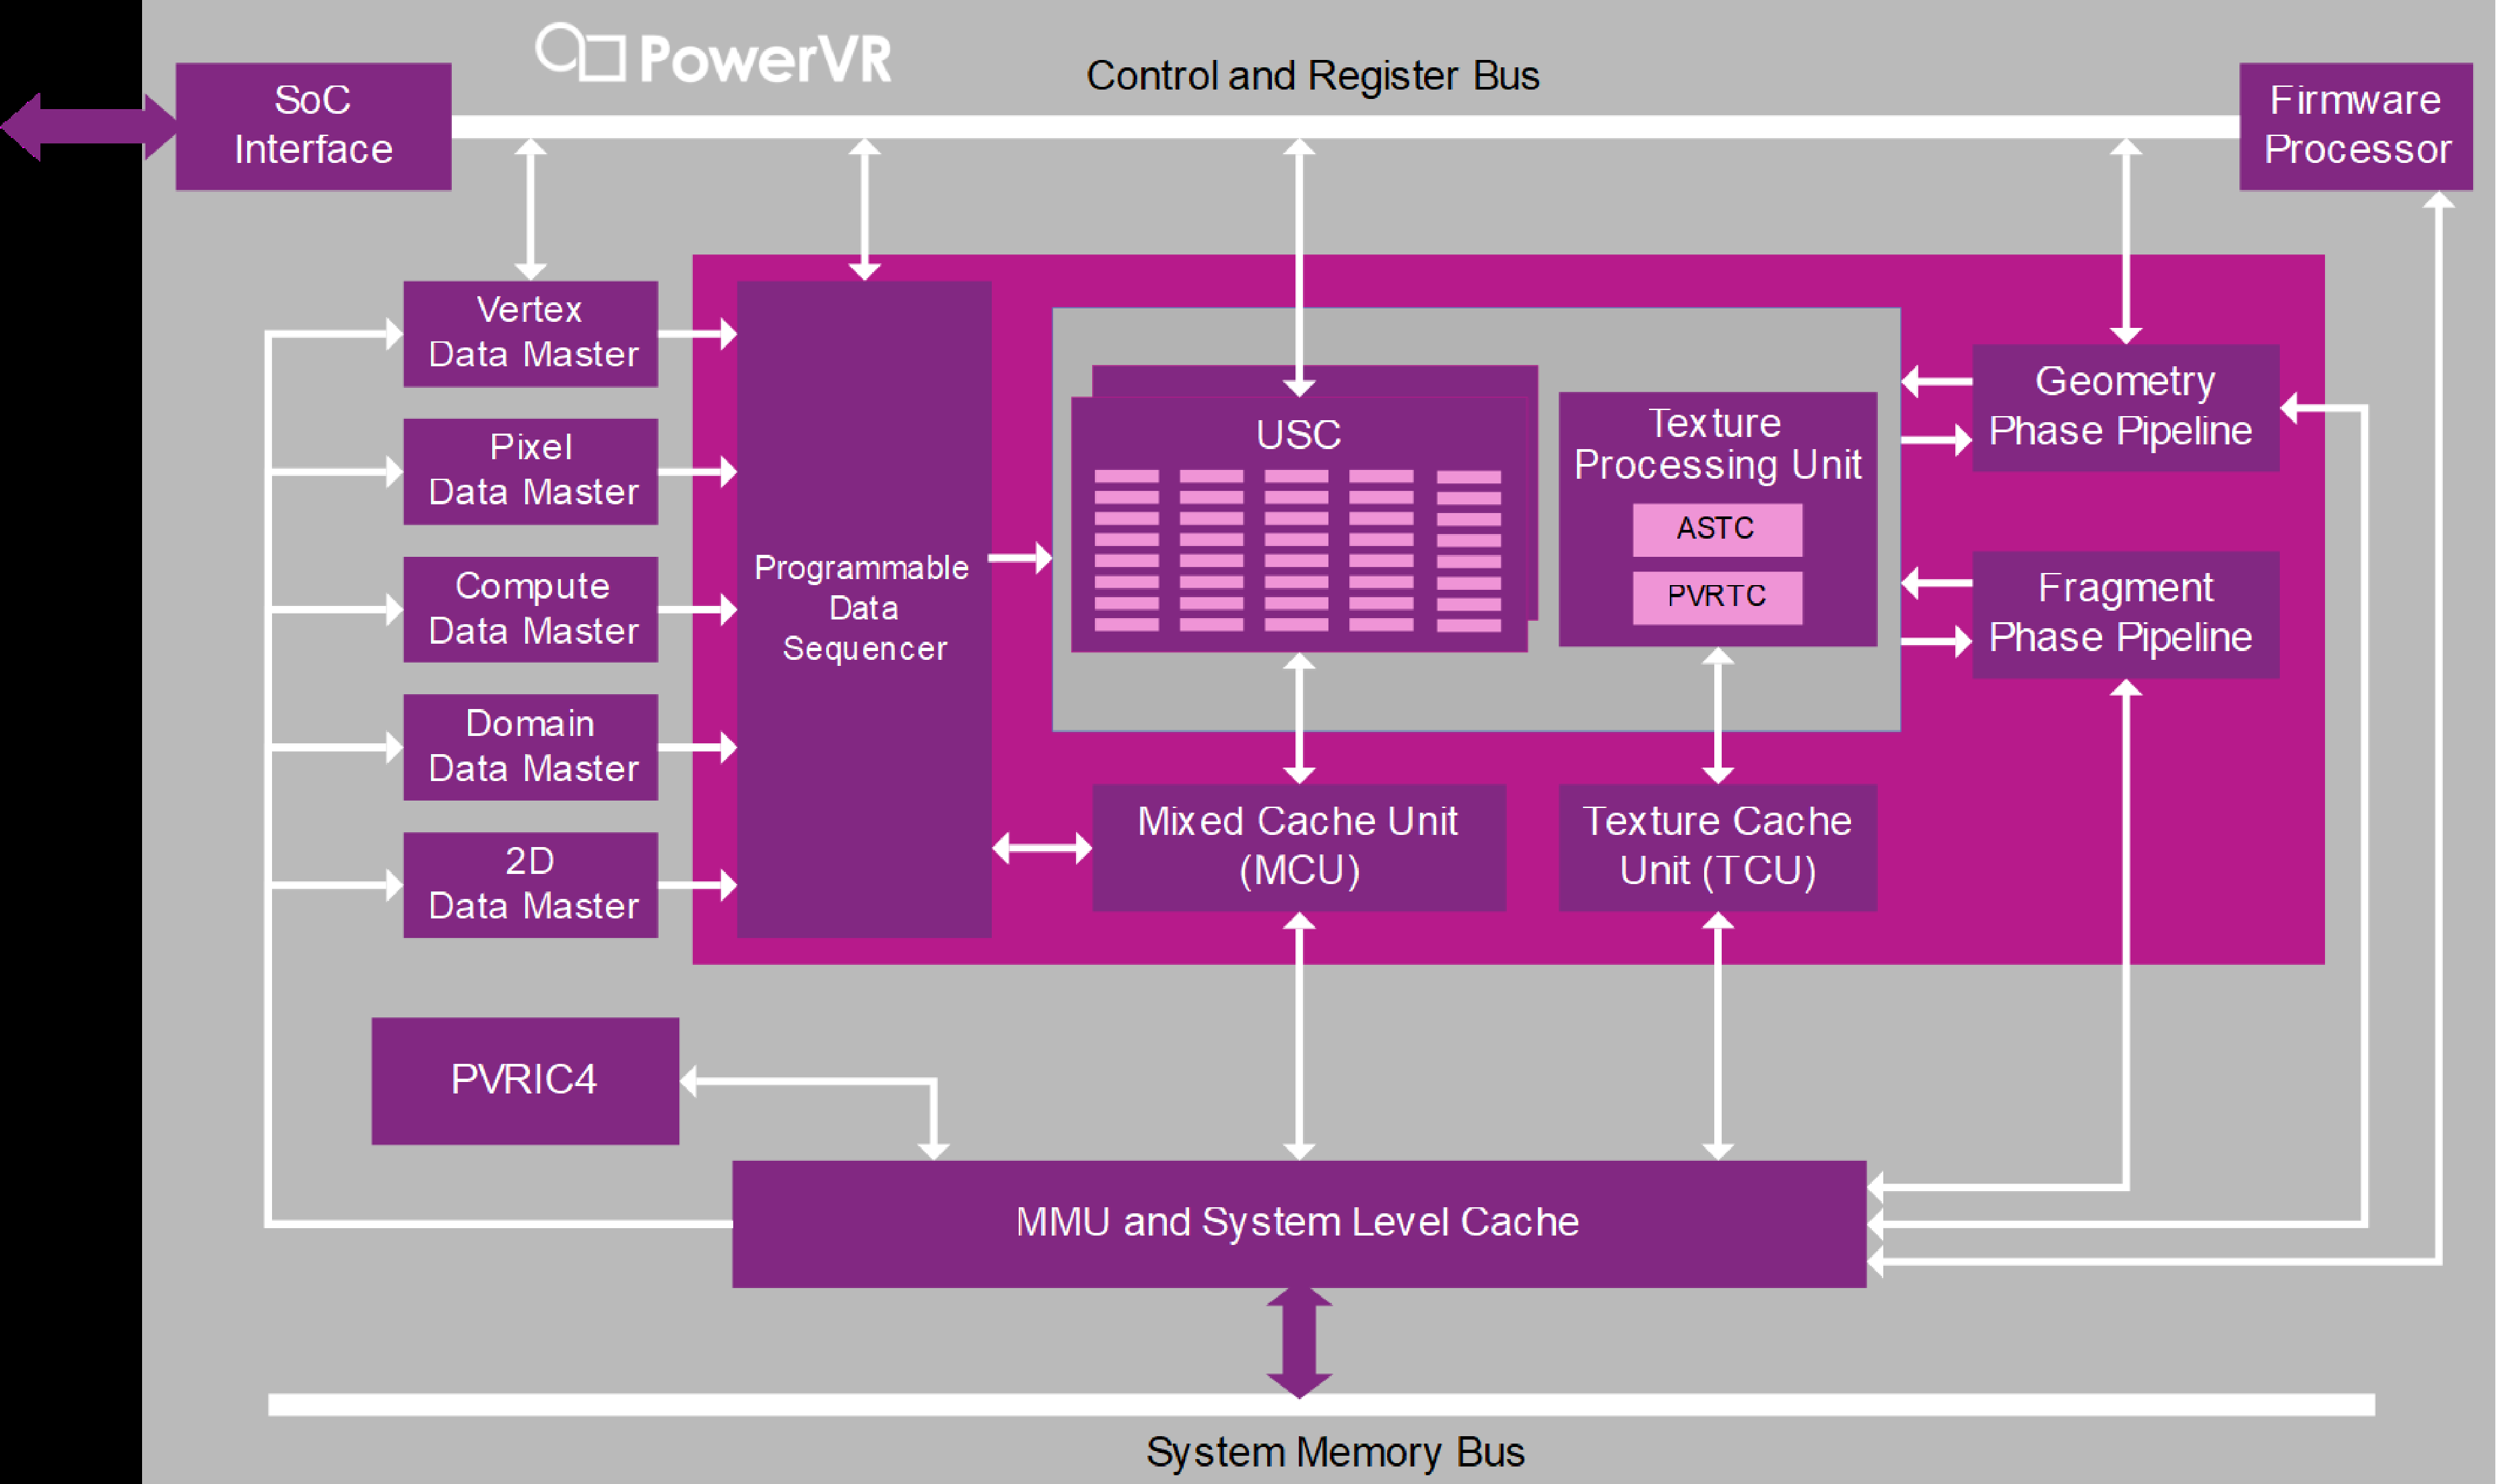
\includegraphics[valign=t,width=0.99\textwidth]{pictures/ImTech_Type-3_4-architecture-overview.pdf}\\
  Общий вид
    \end{center}
  \end{minipage}
  \begin{minipage}[t]{0.49\textwidth}
    \begin{center}
  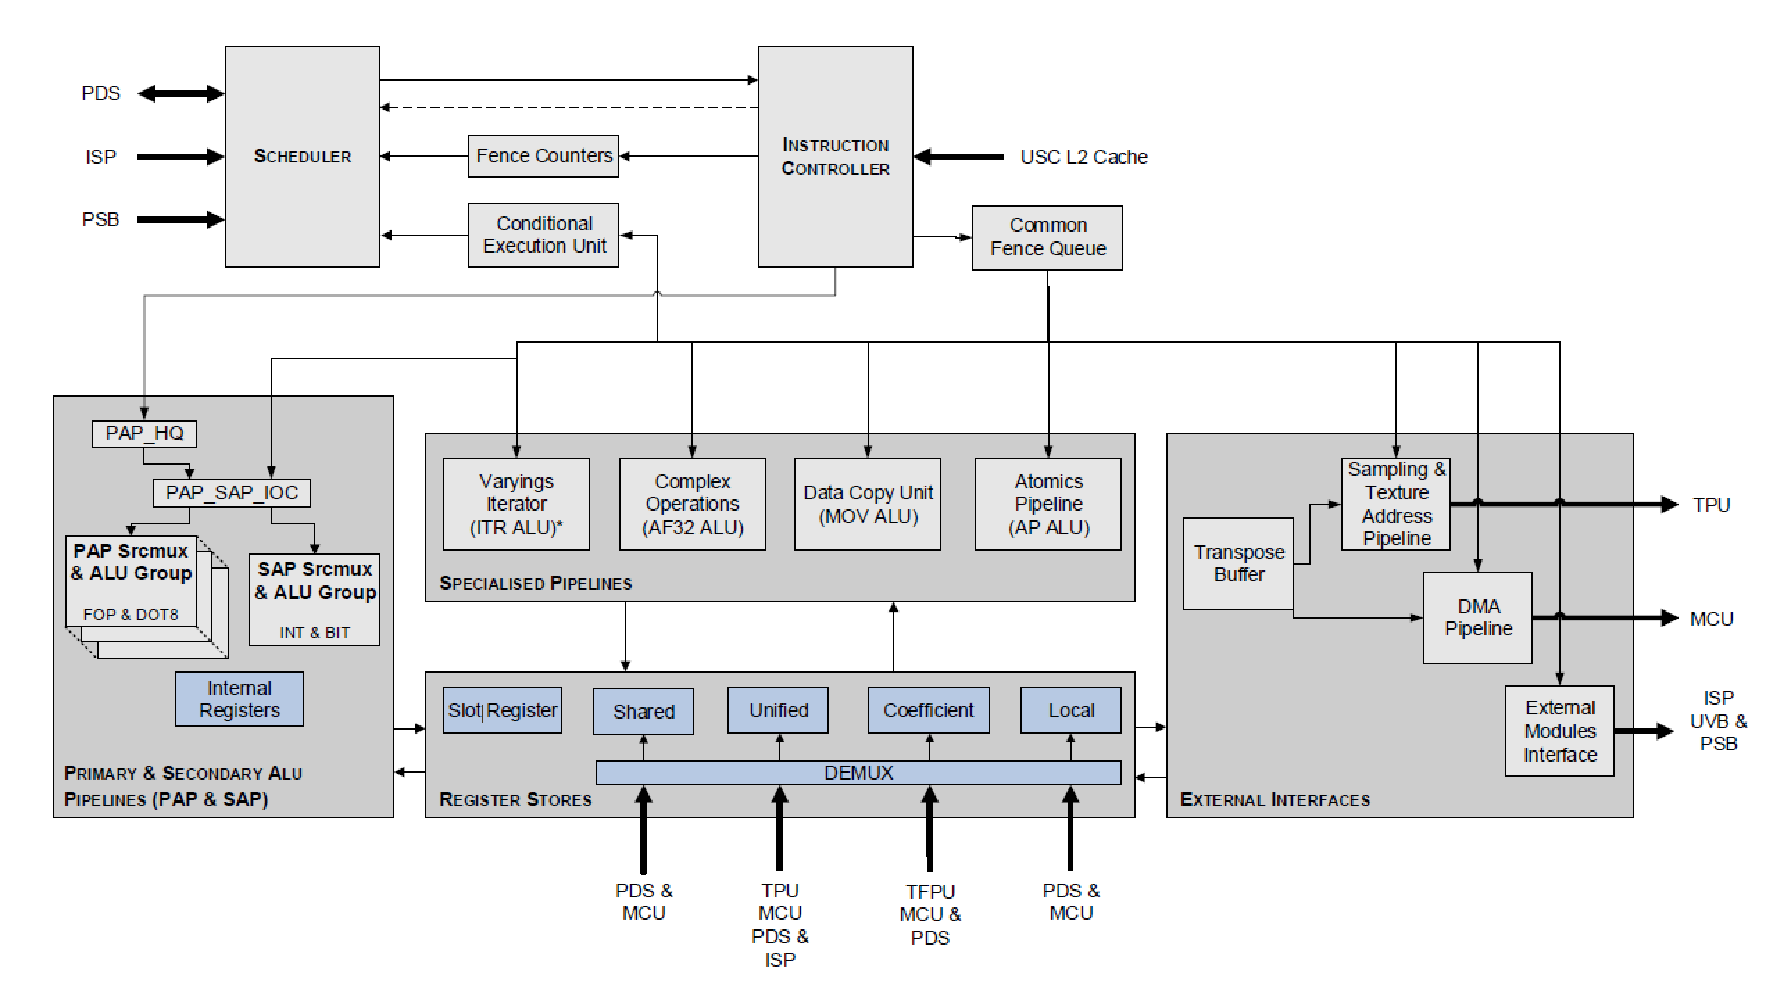
\includegraphics[valign=t,width=0.99\textwidth]{pictures/ImTech_Type-4-architecture-unified-shading-cluster.pdf}\\
  Детали Unified Shading Cluster
\end{center}
\end{minipage}
\end{frame}


\begin{frame}[fragile]
  \frametitle{Микроархитектура RISC-V GPGPU Vortex\footnote{Примерно то, с чем другие некоторые столкнутся на школе}\textsuperscript{,}\footnote{Изображение со страницы проекта: \url{https://github.com/vortexgpgpu/vortex/blob/master/docs/microarchitecture.md
  }}}
  \vspace{-0.7cm}
    \begin{center}
  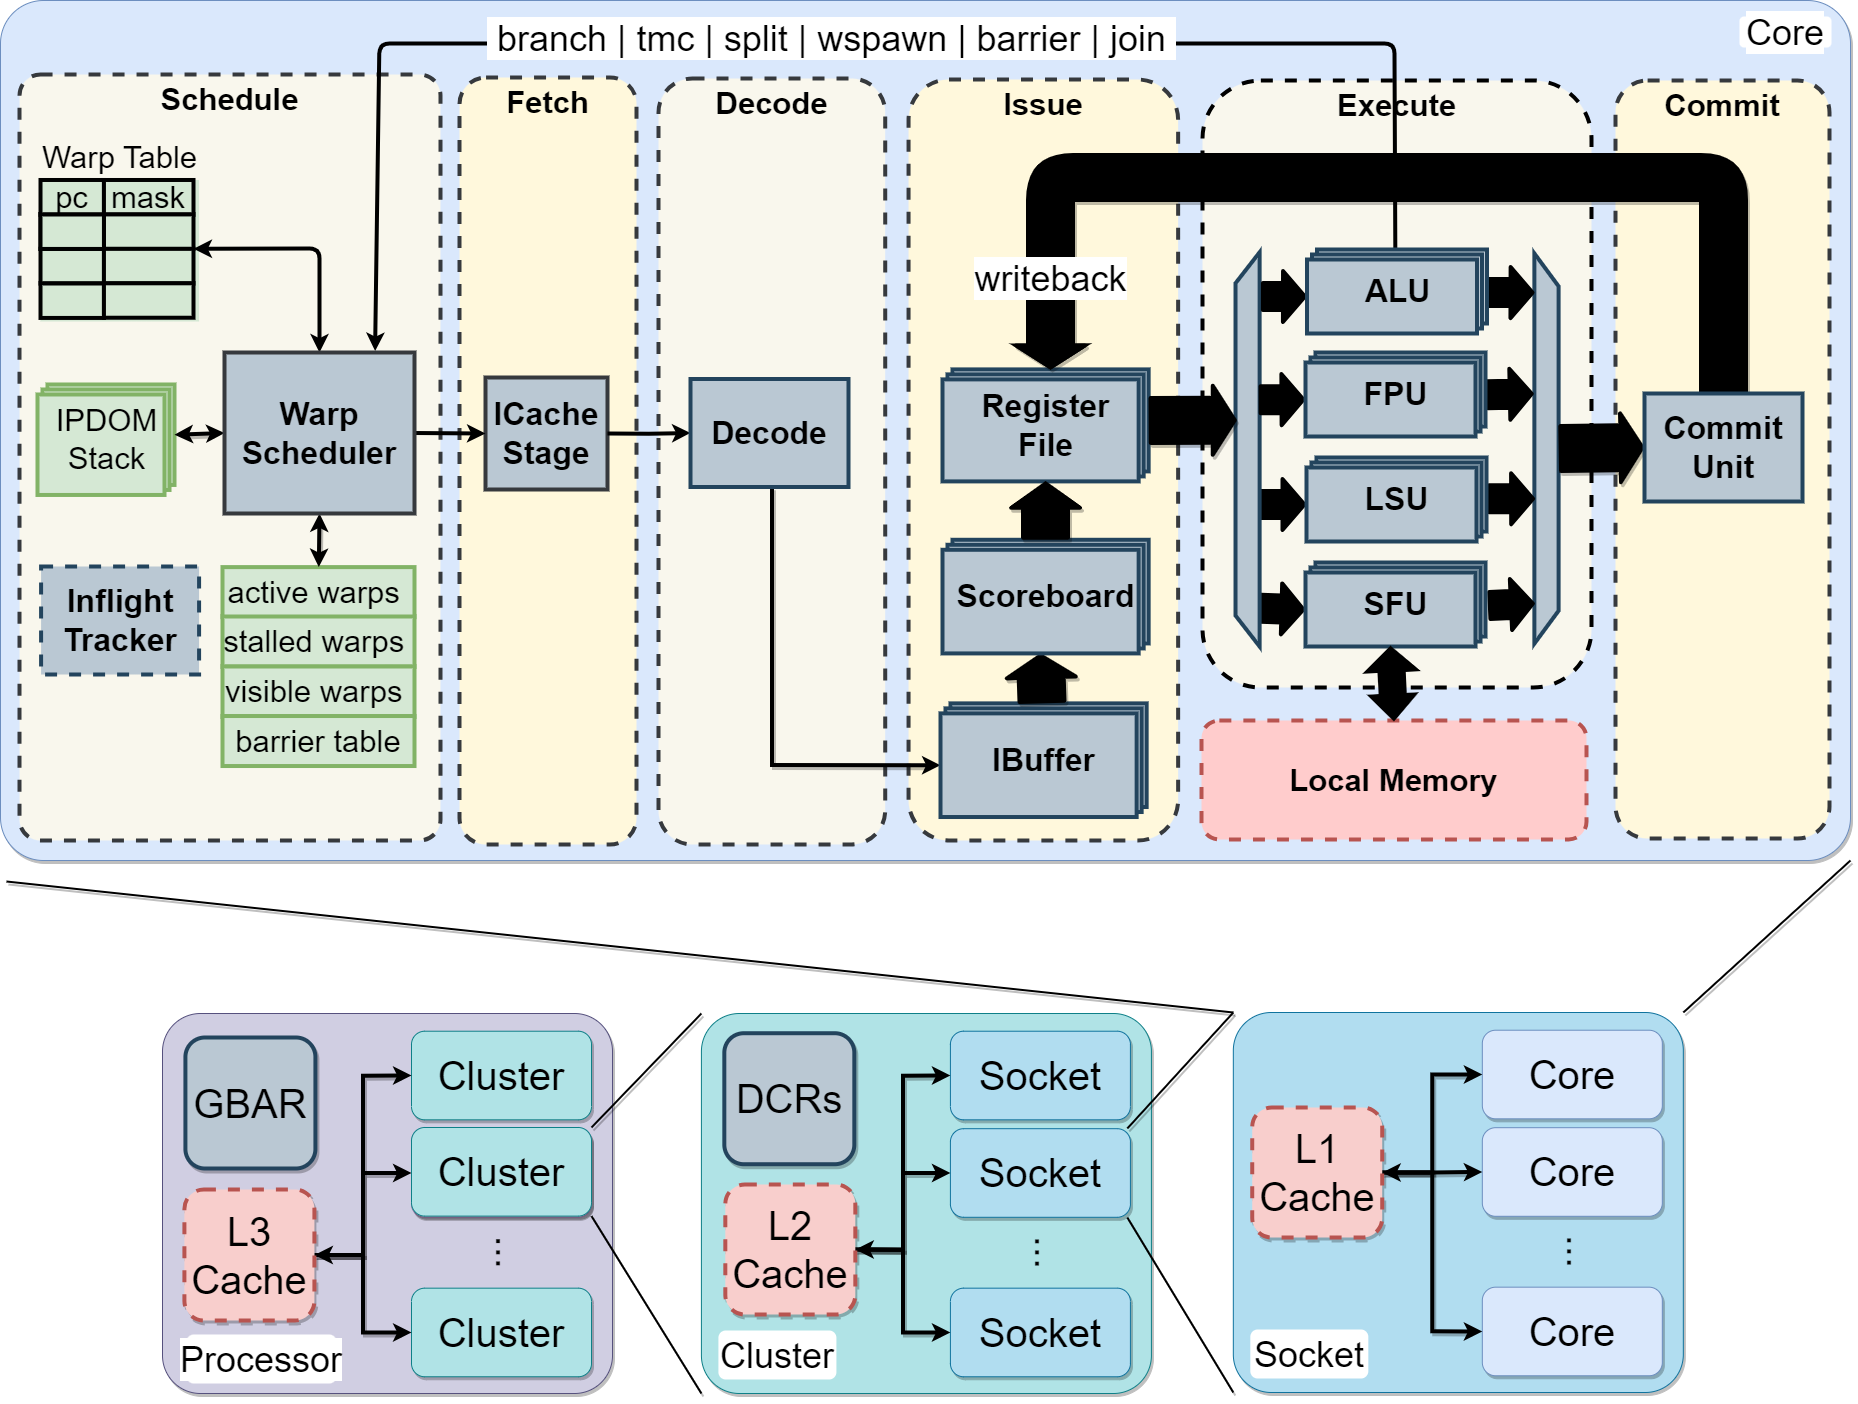
\includegraphics[valign=t,width=0.55\textwidth]{pictures/vortex_microarchitecture.png}\\
  
\end{center}

\end{frame}

\begin{frame}[fragile]
  \frametitle{OpenCL: Open Computing Language \hfill \vspace{-0.1cm}
\includegraphics[height=0.7cm]{pictures/OpenCL_CMYK_Apr20.eps}}
  \begin{itemize}
    \item \href{https://www.khronos.org/opencl/}{Khronos\footnote{Консорциум для работы над открытыми стандартами в области параллельных вычислений, машинного обучения, компьютерной графики: больше 180 организаций, 21 стандарт. \url{https://www.khronos.org/}.}}: <<Open Standard for \textbf{Parallel} Programming of \textbf{Heterogeneous} Systems>>
    \begin{itemize}
      \item \underline{Многоядерные CPU}
      \item \underline{\textbf{Графические ускорители, GPGPU}}
      \item Программируемые логические интегральные семы, ПЛИС/FPGA
      \item Процессоры для цифровой обработки сигналов, DSP
      \item \ldots
    \end{itemize}
    \item Активно разрабатывается и используется
    \begin{itemize}
      \item Intel, Google, Nvidia, AMD, Imagination Technologies, \ldots
      \item OpenCV, FFmpeg, ViennaCL, GNU Octave, Matlab, \ldots
    \end{itemize}
  \item Версии стандарта
  \begin{itemize}
    \item 1.2: 2011 год, обязательная база для 3.0
    \item 2.x: 2013 год, <<откатили>> в 3.0
    \item 3.0: 2020 год, 3.0.17 в октябре 2024
  \end{itemize} 
  \end{itemize}
\end{frame}

\begin{frame}[fragile]
  \frametitle{OpenCL: структура программы}
  \begin{minipage}[t]{0.7\textwidth}
  \begin{itemize}
    \item \textbf{Часть кода выполняется на центральном процессоре, часть на ускорителе}
    \item Центральный процессор (\textbf{<<хост>>, host})
    \begin{itemize}
      \item Взаимодействие с <<внешним миром>>, подготовка данных, запуск кода на ускорителе
      \item Хочется писать код на <<типичном>> языке программирования
    \end{itemize} 
    \item Ускоритель (\textbf{<<устройство>>, device})
    \begin{itemize}
      \item Обработка данных <<по указке>> центрального процессора
      \item Придётся пользоваться специализированным языком
      \item Процедура, предназначенная для выполнения на ускорителе --- \textbf{<<ядро>>, kernel}\footnotemark
    \end{itemize} 
  \end{itemize}
\end{minipage}
\begin{minipage}[t]{0.28\textwidth}
  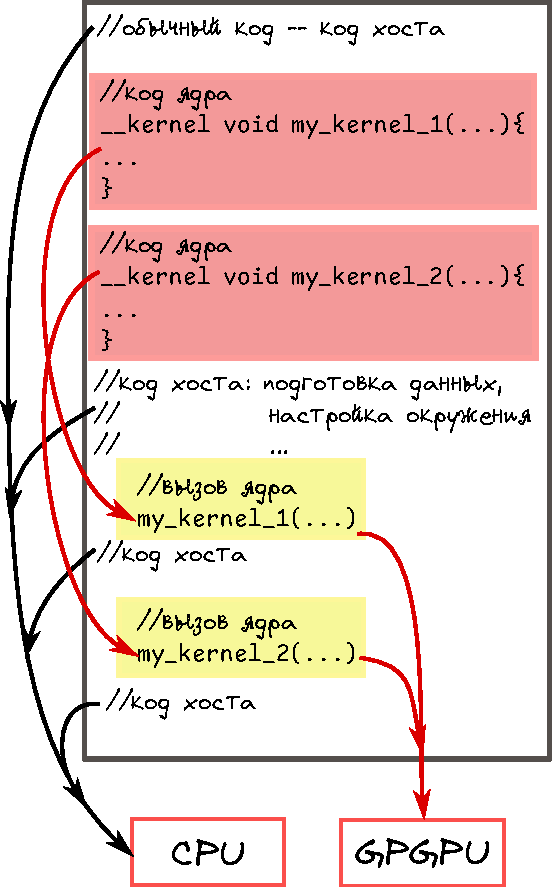
\includegraphics[valign=t,width=\textwidth]{pictures/host-kernel-code.pdf}
\end{minipage}
\footnotetext{OpenCL kernel, CUDA kernel, \ldots }
\end{frame}

\begin{frame}[fragile]
  \frametitle{OpenCL: взаимодействие хоста и устройства}
  \begin{itemize}
    \item Обнаружение, подключение, конфигурация устройств\footnote{ICD-Loader: \url{https://github.com/KhronosGroup/OpenCL-ICD-Loader}}
    \item Управление памятью\footnote{Основной примитив --- буфер: \url{https://registry.khronos.org/OpenCL/specs/3.0-unified/html/OpenCL_API.html\#_buffer_objects}}
    \begin{itemize}
      \item Выделение/освобождение
      \item Контроль доступа и синхронизации между хостом и устройствами
    \end{itemize} 
    \item Выполнение команд 
    \begin{itemize}
      \item Передача данных, запуск ядер, синхронизация, \ldots
      \item Основной интерфейс взаимодействия --- \textbf{очередь команд}\footnote{Command queue: \url{https://registry.khronos.org/OpenCL/specs/3.0-unified/html/OpenCL_API.html\#_command_queues}}
      \begin{itemize}
        \item Неблокирующая: центральный процессор ставит задачи, но не дожидается их исполнения
        \item Нужны дополнительные действия чтобы узнать, когда закончилась определённая задача
        \item In-order: команды выполняются строго друг за другом
        \item Может быть out-of-order
        \item Синхронизация между несколькими очередями возможна, но требует отельной работы
      \end{itemize}
    \end{itemize} 
  \end{itemize}

\end{frame}


\begin{frame}[fragile]
  \frametitle{Язык для написания ядер: OpenCL C/C++}
  \begin{itemize}
    \item C++ for OpenCL language\footnote{В 2.x был OpenCL C++ Kernel Language}
    \item \textbf{OpenCL C language}\footnote{Спецификация: \url{https://registry.khronos.org/OpenCL/specs/3.0-unified/html/OpenCL_C.html}}
    \begin{itemize}
      \item Диалект C99: специальные типы данных\footnote{\scriptsize{\url{https://registry.khronos.org/OpenCL/specs/3.0-unified/html/OpenCL_C.html\#supported-data-types}}}, модификаторы памяти\footnote{\scriptsize{\url{https://registry.khronos.org/OpenCL/specs/3.0-unified/html/OpenCL_C.html\#address-space-qualifiers}}}
      \item JIT-компиляция\footnote{Для переносимости: вендору целевого устройства <<лучше знать>>, как компилировать}, но бывают и AOT решения
      \item Дополнительные библиотеки времени выполнения
      \item Расширения\footnote{Знакомя ситуация, не правда ли?} 
      \begin{itemize}
        \item Предусмотренные cтандартом\footnote{Поискать <<Khronos Extension Specifications>> на \url{https://registry.khronos.org/OpenCL/}}: \texttt{cl\_khr\_fp64, cl\_khr\_int64\_extended\_atomics, \ldots} 
        \item Расширения от вендоров\footnote{Поискать <<Vendor and Multi-Vendor Extension Specifications>> на \scriptsize{\url{https://registry.khronos.org/OpenCL/}}}: \texttt{cl\_nv\_pragma\_unroll, cl\_amd\_fp64, \ldots} 
      \end{itemize}
    \end{itemize}
  \end{itemize}
\end{frame}

\begin{frame}[fragile]
  \frametitle{OpenCL C: параллельность}
  \begin{minipage}[t]{0.5\textwidth}
  \begin{itemize}
    \item Виртуальная решётка (\textbf{NDRange}) <<потоков>> (\textbf{work-items})
    \begin{itemize}
      \item одно-, двух-, трёхмерная
      \item Группировка узлов в рабочие группы (\textbf{work-group}) фиксированного размера
      \item Возможность получить глобальные и локальные координаты <<потока>>
    \end{itemize}
    \item Параметры (размеры) решётки связаны с <<размерами>> обрабатываемых данных
  \end{itemize}
\end{minipage}
\begin{minipage}[t]{0.48\textwidth}
  \begin{center}
    \vspace{-1cm}
  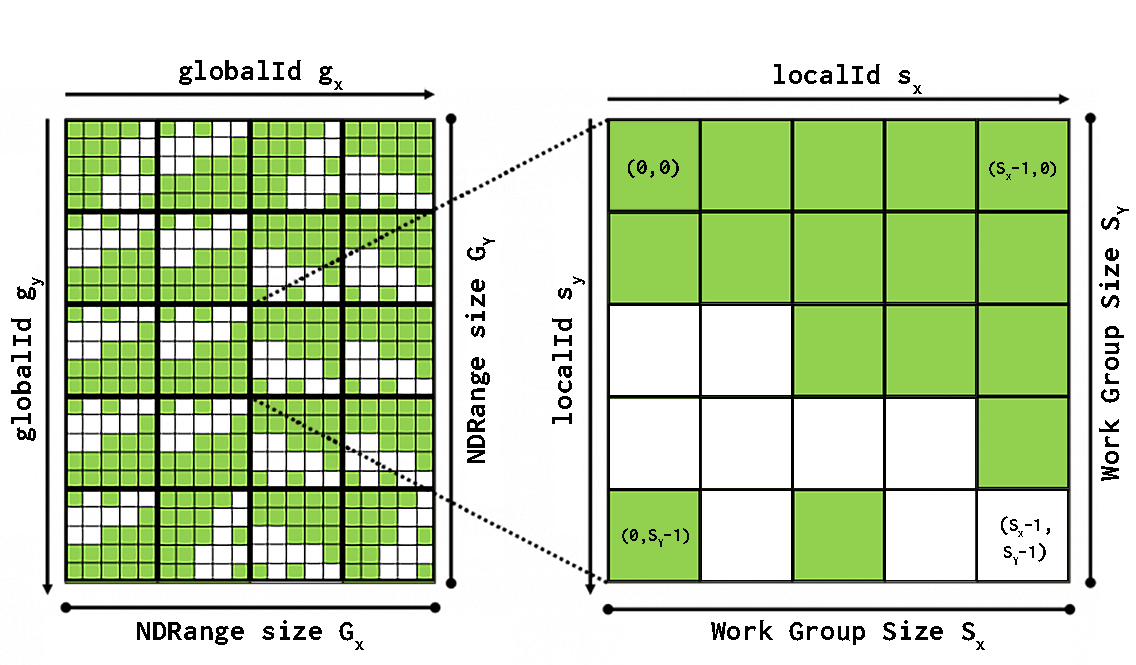
\includegraphics[valign=t,width=\textwidth]{pictures/opeclmap4.png}
  Пример вдухмерной виртуальной решётки\footnotemark
  \end{center}
  \begin{itemize}
    \item \texttt{globalId} --- глобальные координаты
    \item \texttt{localId} --- локальные координаты
  \end{itemize}
\end{minipage}
\footnotetext{Изображение из поста: \url{http://thebeardsage.com/opencl-kernel-space/}}
\end{frame}

%https://registry.khronos.org/OpenCL/specs/3.0-unified/html/OpenCL_API.html#platform-querying-devices

\begin{frame}[fragile]
  \frametitle{И снова проблемы\footnote{<<Шо, опять?>>}}
  \begin{itemize}
    \item[\faQuestion] Как отобразить абстракции OpenCL в реальное устройство?\footnote{При таком-то зоопарке устройств/микроархтектур} 
    \item[\faQuestion] Как писать код, чтобы он показывал хорошую\footnote{Хотелось бы, конечно, максимальную но ...} производительность?    
  \end{itemize}
  \vfill
  \begin{itemize}
    \item[\faFrownO] Придётся писать много вендоро/платформо/device-специфичного кода.
    \begin{itemize} 
      \item[\faSmileO] Кое-что полезное об устройстве можно узнать во время выполнения\footnote{Стандартный API для получения данных об устройстве: \url{https://registry.khronos.org/OpenCL/specs/3.0-unified/html/OpenCL_API.html\#platform-querying-devices}}
      \item[\faMehO] От перебора вороха вариантов в коде всё равно не уйти 
    \end{itemize} 
    \item[\faExclamation] Есть некоторые общие принципы 
  \end{itemize}
\end{frame}

\begin{frame}[fragile]
  \frametitle{Общие принципы работы с очередью команд}
  Помни!
  \begin{itemize}
    \item Постановка задачи в очередь --- накладные расходы
    \item Разные задачи в очереди задействуют разные ресурсы
    \item Одна задача может не утилизировать какой-то ресурс полностью 
    \item Ожидание завершения задачи может привести к потере вычислительного времени
  \end{itemize}
  Потому
  \begin{itemize}
    \item Не дроби ядра
    \item Используй разные очереди или out-of-order\footnote{Там, где это возможно}
    \item Ставь в очередь как можно больше задач\footnote{В разумных пределах} 
    \item Пользуйся тем, что очередь неблокирующая
    \item Уменьшай количество точек синхронизации
  \end{itemize}
\end{frame}

\begin{frame}[fragile]
  \frametitle{Общие принципы работы с памятью}
  Помни!
  \begin{itemize}
    \item Передача данных\footnote{Как между хостом и устройством, так и между устройствами} --- накладные расходы
    \item Память бывает разная: объём и время доступа различаются на порядки
    \item Последовательный доступ --- хорошо, произвольный --- плохо
  \end{itemize}
  Потому
  \begin{itemize}
    \item Помни что где лежит и клади нужное поближе\footnote{Изучи модификаторы памяти в OpenCL C и настройки буферов}
    \item Думай над тем, как представить данные в памяти
    \item Структурируй код ядер так, чтобы минимизировать непоследовательный доступ к памяти
  \end{itemize}
\end{frame}

\begin{frame}[fragile]
  \frametitle{Общие принципы написания ядер}
  Помни!
  \begin{itemize}
    \item Ветвления\footnote{И речь не только об \texttt{if-then-else}} в ядрах --- зло\footnote{К сожалению, иногда --- необходимое зло} 
    \begin{itemize}
      \item Соответствующее неприятное явление называется \textbf{thread divergence} или \textbf{branch divergence}
    \end{itemize}
    \item На аппаратном уровне \underline{\textbf{вполне определённая}}\footnote{В зависимости от вендора: Task, Thread Group, Warp, Wavefront, \ldots} группа <<потоков>> гарантированно выполняет одну инструкцию и рабочая группа как правило отображается в неё
  \end{itemize}
  Потому
  \begin{itemize}
    \item Старайся писать как можно более линейный код
    \begin{itemize}
      \item Иногда ради этого приходится писать несколько ядер
    \end{itemize}
    \item Подбирай размер рабочей группы так, чтобы максимально использовать аппаратные ресурсы
  \end{itemize}
\end{frame}


\begin{frame}[fragile]
  \frametitle{Классический пример\footnote{Материалы из туториала \url{https://cnugteren.github.io/tutorial/pages/page1.html}. Соответствующий код: \url{https://github.com/cnugteren/myGEMM}}}
  \begin{minipage}[t][0.5\textheight]{0.32\textwidth}
    \begin{center}
      \vspace{-1cm}
      Наивная реализация
    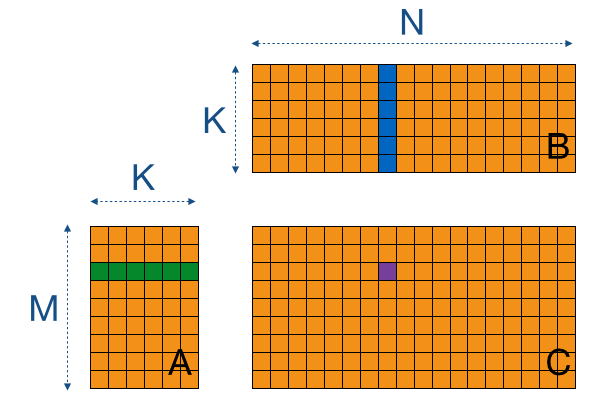
\includegraphics[valign=t,width=\textwidth]{pictures/gemm1.png}
    \vfill
    139 GFLOPS
    \end{center}
  \end{minipage}
  \begin{minipage}[t][0.5\textheight]{0.32\textwidth}
    \begin{center}
      \vspace{-1cm}
      Локальная память
    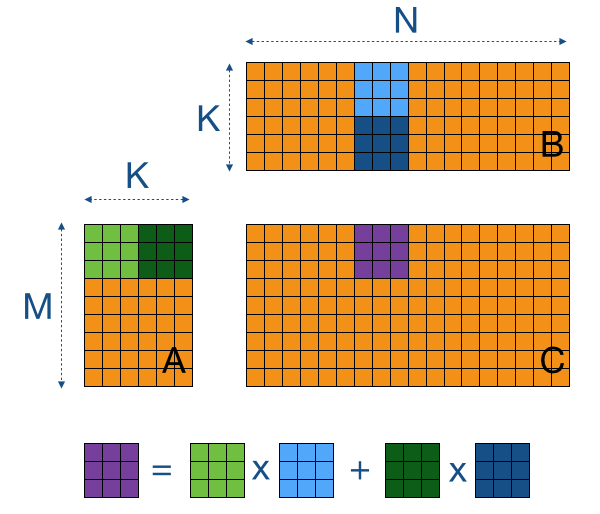
\includegraphics[valign=t,width=\textwidth]{pictures/gemm2a.png}
    \vfill
    373 GFLOPS
  \end{center}
  \end{minipage}
  \begin{minipage}[t][0.5\textheight]{0.32\textwidth}
    \begin{center}
      \vspace{-1cm}
      Регистры
    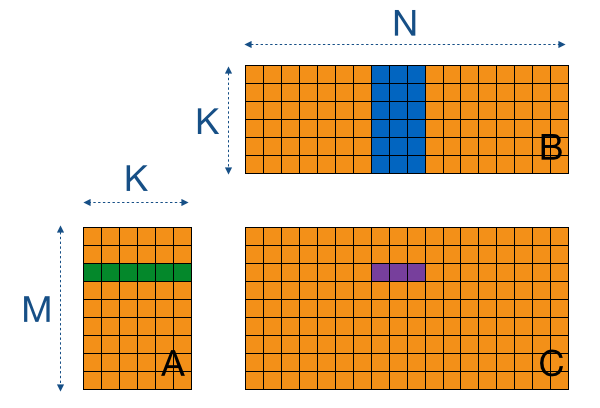
\includegraphics[valign=t,width=\textwidth]{pictures/gemm3.png}
    \vfill
    689 GFLOPS
  \end{center}
  \end{minipage}
  \vfill
  \begin{itemize}
    \item \texttt{cuBLAS} в тех же условиях: 3056 GFLOPS
  \end{itemize}
\end{frame}





\begin{frame}[fragile]
  \frametitle{Немного полезных ссылок}
  \begin{itemize}
    \item \href{https://www.khronos.org/opencl/}{Khronos OpenCL}
    \begin{itemize}
      \item \scriptsize{\url{https://www.khronos.org/opencl/}}
    \end{itemize}
    \item \href{https://enccs.github.io/gpu-programming/}{Курс по разработке под GPGPU от EuroCC National Competence Center Sweden}
    \begin{itemize}
      \item \scriptsize{\url{https://enccs.github.io/gpu-programming/}}
    \end{itemize}
    \item \href{https://blog.imaginationtech.com/a-quick-guide-to-writing-opencl-kernels-for-rogue/}{OpenCL для ускорителей от Imagination Technologies}
    \begin{itemize}
      \item \scriptsize{\url{https://blog.imaginationtech.com/a-quick-guide-to-writing-opencl-kernels-for-rogue/}}
    \end{itemize}
    \item \href{https://docs.imgtec.com/performance-guides/compute-recommendations/html/index.html}{Рекомендации разработчику под ускорители от Imagination Technologies}
    \begin{itemize}
      \item \scriptsize{\url{https://docs.imgtec.com/performance-guides/compute-recommendations/html/index.html}}
    \end{itemize}
    \item \href{https://cvw.cac.cornell.edu/gpu-architecture}{Cornell University, Understanding GPU Architecture}
    \begin{itemize}
      \item \scriptsize{\url{https://cvw.cac.cornell.edu/gpu-architecture}}
    \end{itemize}
    \item \href{https://istina.msu.ru/publications/book/76785028/}{Антонюк В. А. OpenCL Открытый язык для параллельный программ, учебное пособие, 2017.}
    \begin{itemize}
      \item \scriptsize{\url{https://istina.msu.ru/publications/book/76785028/}}
    \end{itemize} 
  \end{itemize}
\end{frame}

% https://docs.imgtec.com/performance-guides/compute-recommendations/html/topics/introduction/introduction.html
% https://docs.imgtec.com/performance-guides/compute-recommendations/html/topics/architecture/overview.html#id11
\end{document}
